\documentclass[10pt]{article}
\usepackage{sdss2020} % Uses Times Roman font (either newtx or times package)
\usepackage{url}
\usepackage{latexsym}
\usepackage{amsmath, amsthm, amsfonts}
\usepackage{algorithm, algorithmic}  
\usepackage{multirow,graphicx}
\usepackage[flushleft]{threeparttable}
\usepackage[T1]{fontenc}
\usepackage{booktabs}
\usepackage{siunitx} 
\graphicspath{ {./Images/} }

\newcolumntype{L}[1]{>{\raggedright\let\newline\\\arraybackslash\hspace{0pt}}m{#1}}
\newcolumntype{C}[1]{>{\centering\let\newline\\\arraybackslash\hspace{0pt}}m{#1}}
\newcolumntype{R}[1]{>{\raggedleft\let\newline\\\arraybackslash\hspace{0pt}}m{#1}}
\renewcommand{\thesubsection}{\thesection.\Alph{subsection}}

\title{Modeling Opening Weekend Box Office Revenue for Domestic Movies, 2005-2007}

\author{
  C. Logue \\
  Georgetown University \\
  Washington, DC \\
\\\And
  P. Mernagh \\
  Georgetown University \\
  Washington, DC \\
\\\And
  Z. Holden \\
  Georgetown University \\
  Washington, DC \\
\\}

\begin{document}
\maketitle

\section{Introduction}
The aim of this study was to explore what factors made films successful in attracting viewers to theater releases. Our primary motivation was personal interest as life-long “movie-buffs,” with extensive experience at the box office. Furthermore, we were encouraged by the wealth of free and publicly available data on films and their performance in theaters.
To demarcate bounds, we decided to evaluate film releases prior to the rise of streaming—we felt it would be very difficult to account for the potential impacts of streaming on consumer behavior and the box office industry at large. In this vein—and to control for any shifting societal, political, economic or inflationary factors—we chose to focus on films released between 2005 and 2007. We chose to study feature-length films released in domestic theaters, filtering out short films, and keeping in line with our own experience. Finally, we decided to limit the timeframe of performance to the industry-standard “opening weekend,” allowing us to best control for variance in theater runs.
Provided data availability, we determined revenue would be the best target variable to quantify viewership, assuming ticket prices were more or less equivalent across theaters. 
Having reflected on our own experiences, we felt potentially important covariates would be centered around the “intrinsic” characteristics of each film: the business elements behind its production, its subject matter, its prequels (if any), its cast actors, and its hired crew.  
\section{Data}
\subsection{Collection}
We gathered our data from The Movie Database and Box Office Mojo. The Movie Database (“TMDB”) is a user-generated database of film and television, consisting of information and ratings on almost one million films internationally. Box Office Mojo is a subsidiary of IMDB which reports on domestic and international box-office statistics as far back as 1977.
The Movie Database (“TMDB”) REST API was queried for English-language films distributed from 2005 to 2007, then cross-referenced with Box Office Mojo’s domestic opening-weekend statistics. The resulting initial dataset comprised 527 films, including data on: release date, opening weekend performance (e.g. revenue, theater distribution), film characteristics (e.g. genre, sequels), and production (e.g. budget, production companies). As a user-generated platform, TMDB also provided the community’s aggregate film ratings, along with the quantity of submitted votes. These latter features were initially considered as candidates for modeling but subsequently dropped, given the timing of user-submission couldn’t be controlled for. The TMDB API was then queried for supplemental information on the production, cast, and crew. This included features quantifying: the production headcount (e.g. size of writer dept., size of producing dept.), the experience of cast and crew (e.g. number of films the director had previously directed), the reputation of cast and crew (e.g. the median rating of films the writers had previously written), the size of the producing studio (e.g. independent or major), and if the screenplay was based on a prior work (e.g. novel). This exercise effectively doubled our features, with the aim to capture the human element of talent in film production.


\subsection{Cleansing}
According to the Screen Actors Guild\footnote{https://www.sagawards.org/awards/rules-eligibility/eligibility-criteria}, a feature-length film is defined at a minimum threshold of 60 minutes. Observations not meeting this runtime were dropped, along with films erroneously duplicated under different identifiers. In the feature space, we eliminated any irrelevant identifiers, and features beyond the scope of our observation. This included performance metrics recorded concurrently or after our target variable: revenue, opening weekend’s percent of total revenue, and opening theaters. This also included any user-generated features on TMDB mentioned above, including popularity and user ratings. Finally, the names of writers and directors were dropped, given the nominal features were far too granular to appropriately account for, instead opting to design aggregate features to proxy for experience and reputation. 
All missing values were checked against base data to confirm they weren’t development errors. Missing values deemed “reasonable,” i.e. indicating a lack of experience, were filled with a value of zero, and then proxied within a generated binary indicator. Missing values deemed collection errors were simply imputed with their median value. 
The primary nominal features were problematically encoded as a series of nested dictionaries within lists. These nominal features were painstakingly “unwrapped”, then one-hot encoded into binary columns for each level. Features of significance and reasonable size were left in this form; such as genre, which had anywhere from one to six assignments per film. Other features such as production studios, countries filmed in, and origin country were either consolidated into more reasonable sized groups, or transformed into more meaningful form. For example, films in the dataset had been shot in 32 countries; these countries were one-hot encoded, and grouped by continent. There were, however, far more unique production studios involved; these were classified as “major” or “independent” studios, then aggregated into a “percent\_independent” feature along with a binary indicator. The only exception to this exercise was the release date of the film, which we grouped into seasonal or monthly subsets. 
The output, ultimately, of this exercise was a 511-observation dataset, with 73 features describing the “intrinsic” components of film we first sought to characterize.

\subsection{Summary Statistics}
Summary statistics for continuous features are as follows:
\begin{table}[H]
\centering
\caption{Summary Statistics (n = 511)\label{summary_stats}}
\begin{tabular}{lrrr}
\toprule
 & mean & min & max \\
\midrule
opening\_revenue (\$MM) & 14.75 & 0.01 & 151.12 \\
budget (\$MM) & 42.88 & 0.00 & 300.00 \\
runtime & 107.33 & 68.00 & 187.00 \\
num\_prod\_cos & 1.56 & 0.00 & 7.00 \\
previous\_film\_rating & 0.75 & 0.00 & 8.02 \\
cast\_xp\_median & 26.45 & 0.00 & 93.00 \\
cast\_rating\_max & 9.38 & 0.00 & 10.00 \\
writer\_xp\_median & 11.26 & 0.00 & 136.00 \\
writer\_xp\_sum & 27.87 & 0.00 & 366.00 \\
writer\_rating\_median & 5.22 & 0.00 & 10.00 \\
writer\_rating\_max & 6.57 & 0.00 & 10.00 \\
production\_room & 16.71 & 1.00 & 100.00 \\
writers\_room & 2.84 & 1.00 & 26.00 \\
sound\_room & 13.59 & 1.00 & 70.00 \\
crew & 96.05 & 2.00 & 573.00 \\
\bottomrule
\end{tabular}
\end{table}

Counts of films by release month and by genre are found in Tables \ref{month_distribution} and \ref{genre_count}, respectively.

\section{Methods}
\subsection{Baseline Model}
We initially select budget (continuous), series (binary), number of production companies (continuous), runtime (continuous), and season (categorical) to establish a baseline model, with season categorized as Winter (Jan-Feb), Spring (Mar-Apr), Summer (May-Aug), Fall (Sep-Oct), and Holiday (Nov-Dec). The relationships between these predictors and opening revenue are visually examined. From pairs plots of the continuous predictors, budget and opening revenue seem positively, linearly related. There is no apparent relationship between opening revenue and the number of production companies or the runtime of the movie. No significant pairwise correlation appears between the predictors; each predictor displays wide variability, with budget and opening revenue both highly skewed right. Spring, summer, and holiday seasons appear to be associated with higher opening revenue on average, though this is skewed, especially by releases grossing over \$50M. Movies that are part of a series also appear associated with higher opening revenue on average. Initially, a model incorporating all variables produces $R^2_a$ around 0.6, but demonstrates clear heteroscedasticity of residuals. A square-root transformation noticeably stabilizes the variance, and establishes a baseline model, for which we perform residual diagnostics. Both DFFITS and DFBETAS analyses are considered to identify potentially influential observations. VIF analysis is also performed. 

\subsection{Alternate Models}
We then attempt to improve upon the baseline by incorporating variables from our secondary set. We also consider interactions between different genres, and between months and genres. An automated approach taken is backwards elimination, including all interactions between genre pairs and between months and genres. Models are fit successively, dropping the least significant predictor. This process identifies a model achieving $R^2_a$ of 0.75, with noticeable heteroscedasticity and very high multicollinearity, and is not considered further. In parallel, we examine the effect or non-effect of adding individual predictors or classes of predictors, including an exhaustive analysis of the “indie” status of a film, and considering scenarios where indie and non-indie production companies collaborated.

\section{Results}
After scaling budget and opening revenue to millions of dollars for easier interpretation, the baseline model specification is:

\begin{table}[H]
\centering
  \begin{threeparttable}
   \scriptsize
    \caption{Baseline Model}
	\begin{tabular}{lrrrrr}
	\toprule
	                                    & coef & t & P>|t| & 0.025 & 0.975 \\
	\midrule
	const          &       2.9980       &     6.799  &         0.000        &        2.132    &        3.864     \\
	budget         &       0.0330       &    18.651  &         0.000        &        0.030    &        0.036     \\
	is\_series     &       1.2225       &     5.974  &         0.000        &        0.820    &        1.624     \\
	num\_prod\_cos &      -0.2793       &    -3.905  &         0.000        &       -0.420    &       -0.139     \\
	runtime        &      -0.0027       &    -0.652  &         0.514        &       -0.011    &        0.005     \\
	is\_spring     &      -0.3056      &    -1.328  &         0.185        &       -0.758    &        0.147     \\
	is\_summer     &      -0.4470       &    -2.143  &         0.033        &       -0.857    &       -0.037     \\
	is\_fall       &      -1.0822      &    -5.008  &         0.000        &       -1.507    &       -0.658     \\
	is\_holiday    &      -1.0853       &    -4.587  &         0.000        &       -1.550    &       -0.620     \\
	\bottomrule
	\end{tabular}
    \begin{tablenotes}
      \scriptsize
      \item $R^2_a$ = 0.54
    \end{tablenotes}
  \end{threeparttable}    
\end{table}

An increase of \$1 million in the film’s budget is associated with an expected increase of \$33 thousand in the square root of opening revenue, all else held equal. Movies that belong to a series are associated with higher opening weekend revenue, with an estimated increase (in the square root) of \$1.22 million. We do not have significant evidence for runtime influencing opening revenue, while the number of production companies of a movie is associated with an expected decrease in opening revenue. 
Our reference group for the categorical covariate season is Winter, for which the expected (square root) opening revenue is \$3 million. Surprisingly, expected (square root) opening revenue is lower for all the remaining seasons, dropping to \$2.7 million for Spring, \$2.6 million for Summer, and \$1.9 million for the Fall and Holiday seasons. 

Residual diagnostics (Figures \ref{baseline_residuals_vs_fitted}-\ref{baseline_residuals_vs_leverage}) show some heteroscedasticity, which the square-root transformation had improved but not completely remedied. Otherwise, the residuals appear normally distributed, and there appear to be no glaring instances of influential observations.

A DFFITS analysis (Table \ref{dffits}) identifies 32 observations possibly worth investigating. Performing the same regression while dropping these does not significantly change the coefficients, and all are ultimately retained. Since a full DFBETAS analysis is prohibitive, we re-estimate the model after dropping the top observation affecting the estimation of the budget coefficient (Table \ref{dfbetas_budget}), and similarly for the is\_series coefficient (Table \ref{dfbetas_series}). Neither coefficient changes materially, so we retain all observations. Finally, the average VIF is 7, which does not warrant remediation.

Our final model uses forward stepwise selection with continuous covariates, including variables from the secondary set around crew, cast, and director. We create a saturated model, then identify the final retained interactions with backwards elimination and forward selection. For genre-month interaction, we include horror movies released in October and family movies relased in December. For genre-genre interactions, we include rom-com and family-animation effects. Finally, we include a series and sci-fi effect. The final model specification is:

\begin{table}[H]
\centering
  \begin{threeparttable}
  \scriptsize
    \caption{Final Model}
	\begin{tabular}{lrrrrrr}
	\toprule
	                                    & coef & t & P>|t| & 0.025 & 0.975 \\
		\midrule
		const                        &       2.5303       &     8.417  &         0.000        &        1.940    &        3.121     \\
		budget                       &       0.0298       &    15.937  &         0.000        &        0.026    &        0.033     \\
		num\_prod\_cos   &      -0.2908       &    -4.255  &         0.000        &       -0.425    &       -0.156     \\
		crew                         &       0.0034       &     4.268  &         0.000        &        0.002    &        0.005     \\
		cast\_xp\_median             &      -0.0089       &    -2.349  &         0.019        &       -0.016    &       -0.001     \\
		is\_series                   &      -2.2463       &    -1.325  &         0.186        &       -5.579    &        1.086     \\
		previous\_film\_release      &      -0.0003       &    -2.909  &         0.004        &       -0.001    &       -0.000     \\
		previous\_film\_rating       &       0.5557      &     2.205  &         0.028        &        0.060    &        1.051     \\
		first\_time\_directors       &      -0.7159       &    -2.649  &         0.008        &       -1.247    &       -0.185     \\
		is\_feb                      &       0.3944       &     1.251  &         0.212        &       -0.225    &        1.014     \\
		is\_mar                      &       0.3185       &     1.021  &         0.308        &       -0.295    &        0.932     \\
		is\_apr                      &      -0.2979       &    -0.921  &         0.357        &       -0.933    &        0.337     \\
		is\_may                      &      -0.3588       &    -1.038  &         0.300        &       -1.038    &        0.321     \\
		is\_jun                      &       0.1060       &     0.329  &         0.743        &       -0.528    &        0.739     \\
		is\_jul                      &      -0.4237       &    -1.269  &         0.205        &       -1.079    &        0.232     \\
		is\_aug                      &       0.0965       &     0.306  &         0.760        &       -0.524    &        0.717     \\
		is\_sep                      &      -0.7991       &    -2.730  &         0.007        &       -1.374    &       -0.224     \\
		is\_oct                      &      -0.6188       &    -1.925  &         0.055        &       -1.251    &        0.013     \\
		is\_nov                      &      -0.1301       &    -0.396  &         0.692        &       -0.775    &        0.515     \\
		is\_dec                      &      -1.2243       &    -3.671  &         0.000        &       -1.880    &       -0.569     \\
		is\_horror                   &       0.4524      &     2.061  &         0.040        &        0.021    &        0.884     \\
		is\_romance                  &      -0.6347       &    -2.596  &         0.010        &       -1.115    &       -0.154     \\
		is\_comedy                   &       0.0364       &     0.226  &         0.821        &       -0.280    &        0.352     \\
		is\_family                   &      -0.1595       &    -0.780  &         0.436        &       -0.561    &        0.242     \\
		is\_animation                &      -0.3852       &    -0.586  &         0.558        &       -1.676    &        0.906     \\
		is\_sci\_fi                  &      -0.5327       &    -2.122  &         0.034        &       -1.026    &       -0.039     \\
		is\_drama                    &      -0.2956       &    -2.101  &         0.036        &       -0.572    &       -0.019     \\
		is\_oct\_*\_is\_horror       &       1.3565       &     2.474  &         0.014        &        0.279    &        2.434     \\
		is\_dec\_*\_is\_family       &       0.9714       &     1.959  &         0.051        &       -0.003    &        1.946     \\
		is\_comedy\_*\_is\_romance   &       1.2247       &     3.944  &         0.000        &        0.615    &        1.835     \\
		is\_animation\_*\_is\_family &       1.1228       &     1.541  &         0.124        &       -0.309    &        2.555     \\
		is\_series\_*\_is\_sci\_fi   &       1.3973       &     2.423  &         0.016        &        0.264    &        2.531     \\
		\bottomrule
		\end{tabular}
    \begin{tablenotes}
      \scriptsize
      \item $R^2_a$ = 0.63
    \end{tablenotes}  
  \end{threeparttable}    
\end{table}

Residual diagnostics (Figures \ref{final_residuals_vs_fitted}-\ref{final_residuals_vs_leverage}) continue to show some heteroscedasticity, but otherwise appear normally distributed with no notable influential observations. Multicollinearity is slighter worse than the baseline model, with mean VIF around 9. Budget and number of prediction companies have similar effects as in the baseline model, and monthly effects generally mirror the seasonality in the baseline model. 

\section{Discussion}
Various modeling tradeoffs were encountered between the baseline model and alternate models. Creating the categorical variable season led to improved residual diagnostics, while treating each month individually led to more significant interactions. “Indie” status was not significant, either initially modeling it as a binary variable, or treating it continously to capture scenarios where both major and indie studios collaborated on a film, and indie films could be considered as a percentage of total studio contribution. We had expected lower revenue on average in the Winter months, but found the opposite. These have been referred to as the “dump months” in the film industry, effectively a dumping ground for low-potential movies, so our finding was unexpected.

The modeling approach taken (i.e. initially posited predictors vs automated selection) also demonstrated tradeoffs. Both models confirmed budget as an important predictor of opening revenue.
Automated selection led to an increase in $R^2_a$, but tended to worsen heteroscedasticity and introduce multicollinearity. Cross-validation would have paired well with automated selection methods, leading to replicatable results. 

Finally, the use of only classical regression methods was somewhat limiting, for example in initially stabilizing the variance. Further possible avenues of exploration include implementation of cross-validation, additional feature cleansing or engineering, additional data such as popularity metrics or revenue by region, and implementation of modern regression techniques. 

%\bibliographystyle{sdss2020} 
%\bibliography{bibl}

\section*{References}

\flushleft{TMDB data sourced using the TMDB REST API, version 3. The version 3 API documentation can be found at \mbox{https://developer.themoviedb.org/docs/getting-started}.}\\[1em]
\flushleft{Box Office Mojo. (n.d.). \textit{Domestic Box Office For 2005}. \mbox{https://www.boxofficemojo.com/year/2005}}\\[1em]
\flushleft{Box Office Mojo. (n.d.). \textit{Domestic Box Office For 2006}. \mbox{https://www.boxofficemojo.com/year/2006}}\\[1em]
\flushleft{Box Office Mojo. (n.d.). \textit{Domestic Box Office For 2007}. \mbox{https://www.boxofficemojo.com/year/2007}}\\[1em]

\appendix
\clearpage

\section{Supplemental Visualizations}
\begin{figure}[H]
\centering
	\centerline{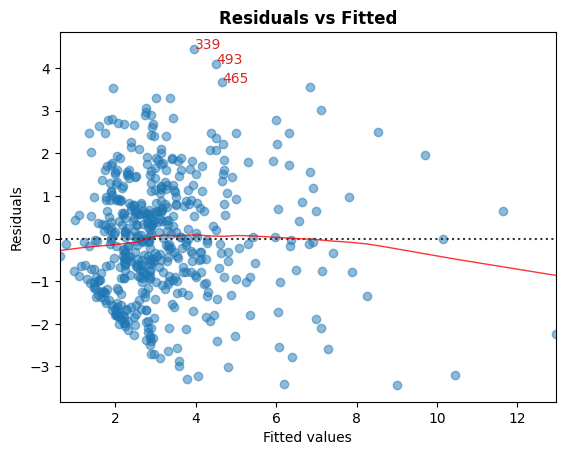
\includegraphics[width=\columnwidth]{baseline_residuals_vs_fitted}}
	\caption{Residuals vs. Fitted Plot, Baseline Model\label{baseline_residuals_vs_fitted}}
\end{figure}

\begin{figure}[H]
\centering
	\centerline{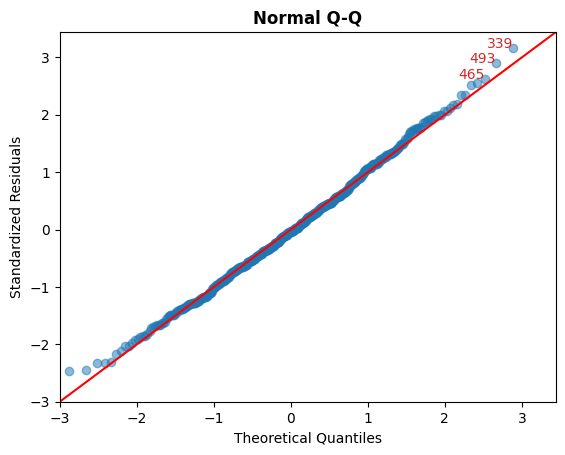
\includegraphics[width=\columnwidth]{baseline_qq}}
	\caption{Q-Q Plot, Baseline Model\label{baseline_qq}}
\end{figure}

\begin{figure}[H]
\centering
	\centerline{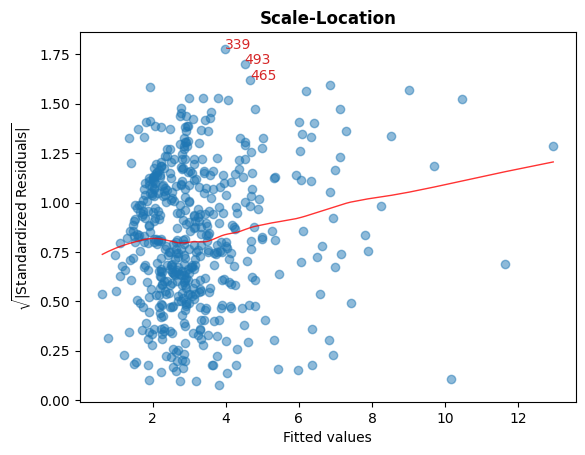
\includegraphics[width=\columnwidth]{baseline_scale_location}}
	\caption{Scale-Location Plot, Baseline Model\label{baseline_scale_location}}
\end{figure}

\begin{figure}[H]
\centering
	\centerline{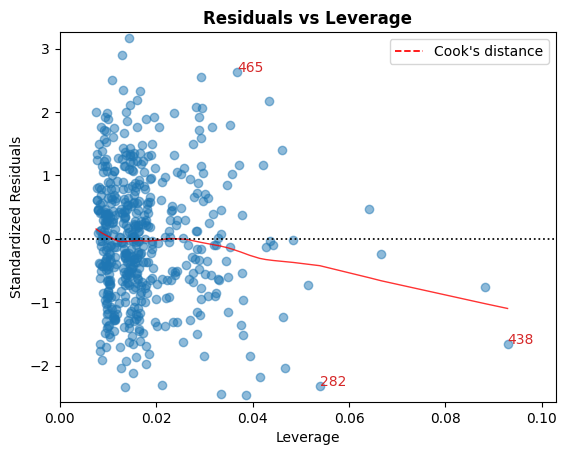
\includegraphics[width=\columnwidth]{baseline_residuals_vs_leverage}}
	\caption{Residuals vs. Leverage Plot, Baseline Model\label{baseline_residuals_vs_leverage}}
\end{figure}









\begin{figure}[H]
\centering
	\centerline{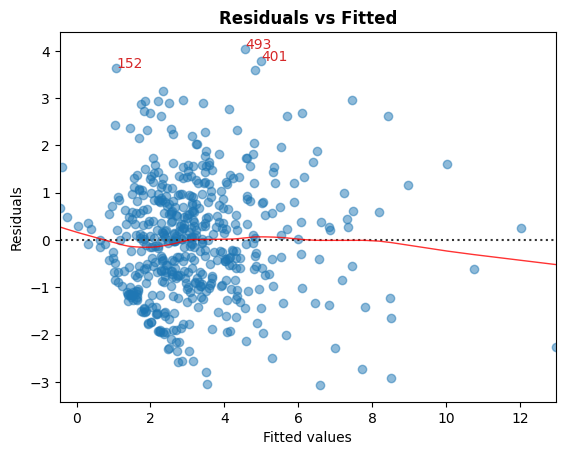
\includegraphics[width=\columnwidth]{final_residuals_vs_fitted}}
	\caption{Residuals vs. Fitted Plot, Final Model\label{final_residuals_vs_fitted}}
\end{figure}

\begin{figure}[H]
\centering
	\centerline{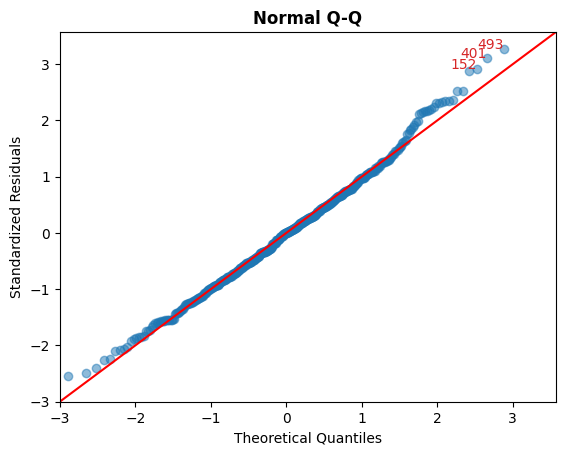
\includegraphics[width=\columnwidth]{final_qq}}
	\caption{Q-Q Plot, Final Model\label{final_qq}}
\end{figure}

\begin{figure}[H]
\centering
	\centerline{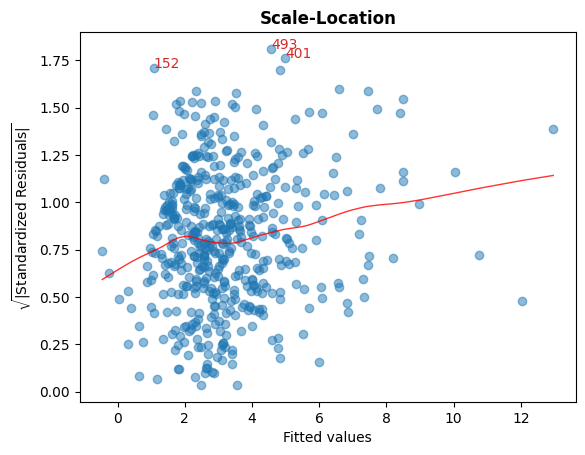
\includegraphics[width=\columnwidth]{final_scale_location}}
	\caption{Scale-Location Plot, Final Model\label{final_scale_location}}
\end{figure}

\begin{figure}[H]
\centering
	\centerline{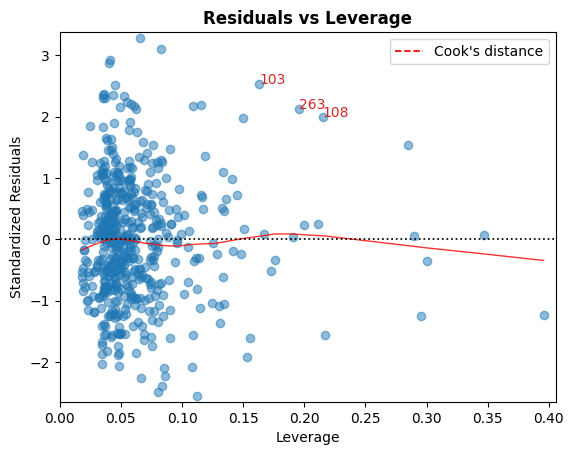
\includegraphics[width=\columnwidth]{final_residuals_vs_leverage}}
	\caption{Residuals vs. Leverage Plot, Final Model\label{final_residuals_vs_leverage}}
\end{figure}



\section{Supplemental Analyses}

\begin{table}[H]
\centering
\caption{Distributions by month of release\label{month_distribution}}
\begin{tabular}{lr}
\toprule
month & count\\
\midrule
is\_jan & 28 \\
is\_feb & 42 \\
is\_mar & 45 \\
is\_apr & 39 \\
is\_may & 31 \\
is\_jun & 43 \\
is\_jul & 35 \\
is\_aug & 45 \\
is\_sep & 71 \\
is\_oct & 50 \\
is\_nov & 37 \\
is\_dec & 45 \\
\bottomrule
\end{tabular}
\end{table}

\begin{table}[H]
\centering
\caption{Count of genres\label{genre_count}}
\begin{tabular}{lr}
\toprule
genre & count  \\
\midrule
is\_adventure & 95 \\
is\_fantasy & 51 \\
is\_animation & 33 \\
is\_drama & 240 \\
is\_horror & 59 \\
is\_action & 103 \\
is\_comedy & 223 \\
is\_history & 25 \\
is\_thriller & 132 \\
is\_crime & 86 \\
is\_documentary & 11 \\
is\_sci\_fi & 39 \\
is\_mystery & 53 \\
is\_music & 17 \\
is\_romance & 107 \\
is\_family & 87 \\
\bottomrule
\end{tabular}
\end{table}

\begin{table}[H]
\caption{DFFITS results, baseline model (Top 10)\label{dffits}}
\begin{tabular}{llr}
\toprule
 obs & release & dffits \\
\midrule
282 & Superman Returns & -0.56 \\
438 & Pirates of the Caribbean: At World's End & -0.53 \\
465 & The Bourne Ultimatum & 0.52 \\
380 & Evan Almighty & -0.50 \\
47 & Harry Potter and the Goblet of Fire & 0.47 \\
102 & Son of the Mask & -0.46 \\
178 & Basic Instinct 2 & -0.45 \\
238 & Letters from Iwo Jima & -0.45 \\
103 & Star Wars: Episode III - Revenge of the Sith & 0.44 \\
339 & 300 & 0.39 \\
\bottomrule
\end{tabular}
\end{table}

\begin{table}[H]
\caption{DFBETAs for budget, baseline model (Top 10)\label{dfbetas_budget}}
\begin{tabular}[t]{l L{0.4\linewidth} rr}
%\begin{tabular}{llr}
\toprule
obs & release & dfbetas & budget (\$MM) \\
\midrule
438 & Pirates of the Caribbean: At World's End & -0.37 & 300.00 \\
380 & Evan Almighty & -0.33 & 175.00 \\
282 & Superman Returns & -0.31 & 223.00 \\
260 & Poseidon & -0.28 & 160.00 \\
401 & I Am Legend & 0.24 & 150.00 \\
419 & Meet the Robinsons & -0.24 & 150.00 \\
238 & Letters from Iwo Jima & 0.23 & 19.00 \\
212 & Flushed Away & -0.23 & 149.00 \\
472 & The Golden Compass & -0.22 & 180.00 \\
452 & Shrek the Third & 0.21 & 160.00 \\
\bottomrule
\end{tabular}
\end{table}

\begin{table}[H]
\caption{DFBETAs for is\_series, baseline model (Top 10)\label{dfbetas_series}}
\begin{tabular}[t]{l L{0.5\linewidth} rr}
\toprule
obs & release & dfbetas & is\_series \\
\midrule
465 & The Bourne Ultimatum & 0.33 & 1 \\
238 & Letters from Iwo Jima & -0.31 & 1 \\
267 & Saw III & 0.29 & 1 \\
102 & Son of the Mask & -0.29 & 1 \\
103 & Star Wars: Episode III - Revenge of the Sith & 0.29 & 1 \\
97 & Saw II & 0.28 & 1 \\
178 & Basic Instinct 2 & -0.26 & 1 \\
449 & Saw IV & 0.26 & 1 \\
47 & Harry Potter and the Goblet of Fire & 0.25 & 1 \\
230 & Jackass Number Two & 0.23 & 1 \\
\bottomrule
\end{tabular}
\end{table}

\section{Replication Data and Code}
\label{a:code}
Replication data and code can be found in the GitHub repo \mbox{https://github.com/cons-code/MATH-5500}.
\end{document}